\section{Introduction}

Human players can learn to play Atari games in minutes~\citep{human_atari_minutes}. However, our best model-free reinforcement learning algorithms require tens or hundreds of millions of time steps -- the equivalent of several weeks of training in real time. How is it that humans can learn these games so much faster? Perhaps part of the puzzle is that humans possess an intuitive understanding of the physical processes that are represented in the game: we know that planes can fly, balls can roll, and bullets can destroy aliens. We can therefore predict the outcomes of our actions. In this paper, we explore how learned video models can enable learning in the Atari Learning Environment (ALE) benchmark~\cite{ale, ale2} with a budget restricted to 100K time steps -- roughly to two hours of a play time.

Although prior works have proposed training predictive models for next-frame, future-frame, as well as combined future-frame and reward predictions in Atari games~\cite{video_prediction,recurrent, video_reward_prediction}, no prior work has successfully demonstrated model-based control via such predictive models that achieve results that are competitive with model-free RL. Indeed, in a recent survey by Machado et al. this was formulated as the following challenge: ``\emph{So far, there has been no clear demonstration of successful planning with a learned model in the ALE}'' (Section 7.2 in \citet{ale2}).


Using models of environments, or informally giving the agent ability to predict its future, has a fundamental appeal for reinforcement learning. The spectrum of possible applications is vast, including learning policies
from the model \citep[Chapter~8]{embed_to_control, deep_spatial, finn2016, ebert, hafner, piergiovanni, rybkin-pertsch,sutton_barto_2017}, capturing important details of the scene \cite{world_models}, encouraging exploration \cite{video_prediction},  creating intrinsic motivation \cite{schmidhuber_formal_theory} or counterfactual reasoning \cite{woulda_coulda_shoulda}.
One of the exciting benefits of model-based learning is the promise to substantially improve sample efficiency of deep reinforcement learning (see Chapter 8 in \cite{sutton_barto_2017}).

Our work advances the state-of-the-art in model-based reinforcement learning by introducing a system that, to our knowledge, is the first to successfully handle a variety of challenging games in the ALE benchmark. To that end, we experiment with several stochastic video prediction techniques, including a novel model based on discrete latent variables. We present an approach, called Simulated Policy Learning (SimPLe), that utilizes these video prediction techniques and trains a policy to play the game within the learned model. With several iterations of dataset aggregation, where the policy is deployed to collect more data in the original game, we learn a policy that, for many games, successfully plays the game in the real environment (see videos on the project webpage \url{https://goo.gl/itykP8}). %\href{https://sites.google.com/view/modelbasedrlatari/home}{dedicated webpage\footnote{\url{https://sites.google.com/view/modelbasedrlatari/home}} with visualizations} of experiments presented in Section \ref{sec:experiments}).

In our empirical evaluation, we find that SimPLe is significantly more sample-efficient than a highly tuned version of the state-of-the-art Rainbow algorithm~\cite{rainbow} on almost all games. In particular, in low data regime of $100$k samples, on more than half of the games, our method achieves a score which Rainbow requires at least twice as many samples. In the best case of {\freeway}, our method is more than 10x more sample-efficient, see Figure \ref{fig:compare_dopamine_ppo}.

\begin{figure*}[t]
\centering
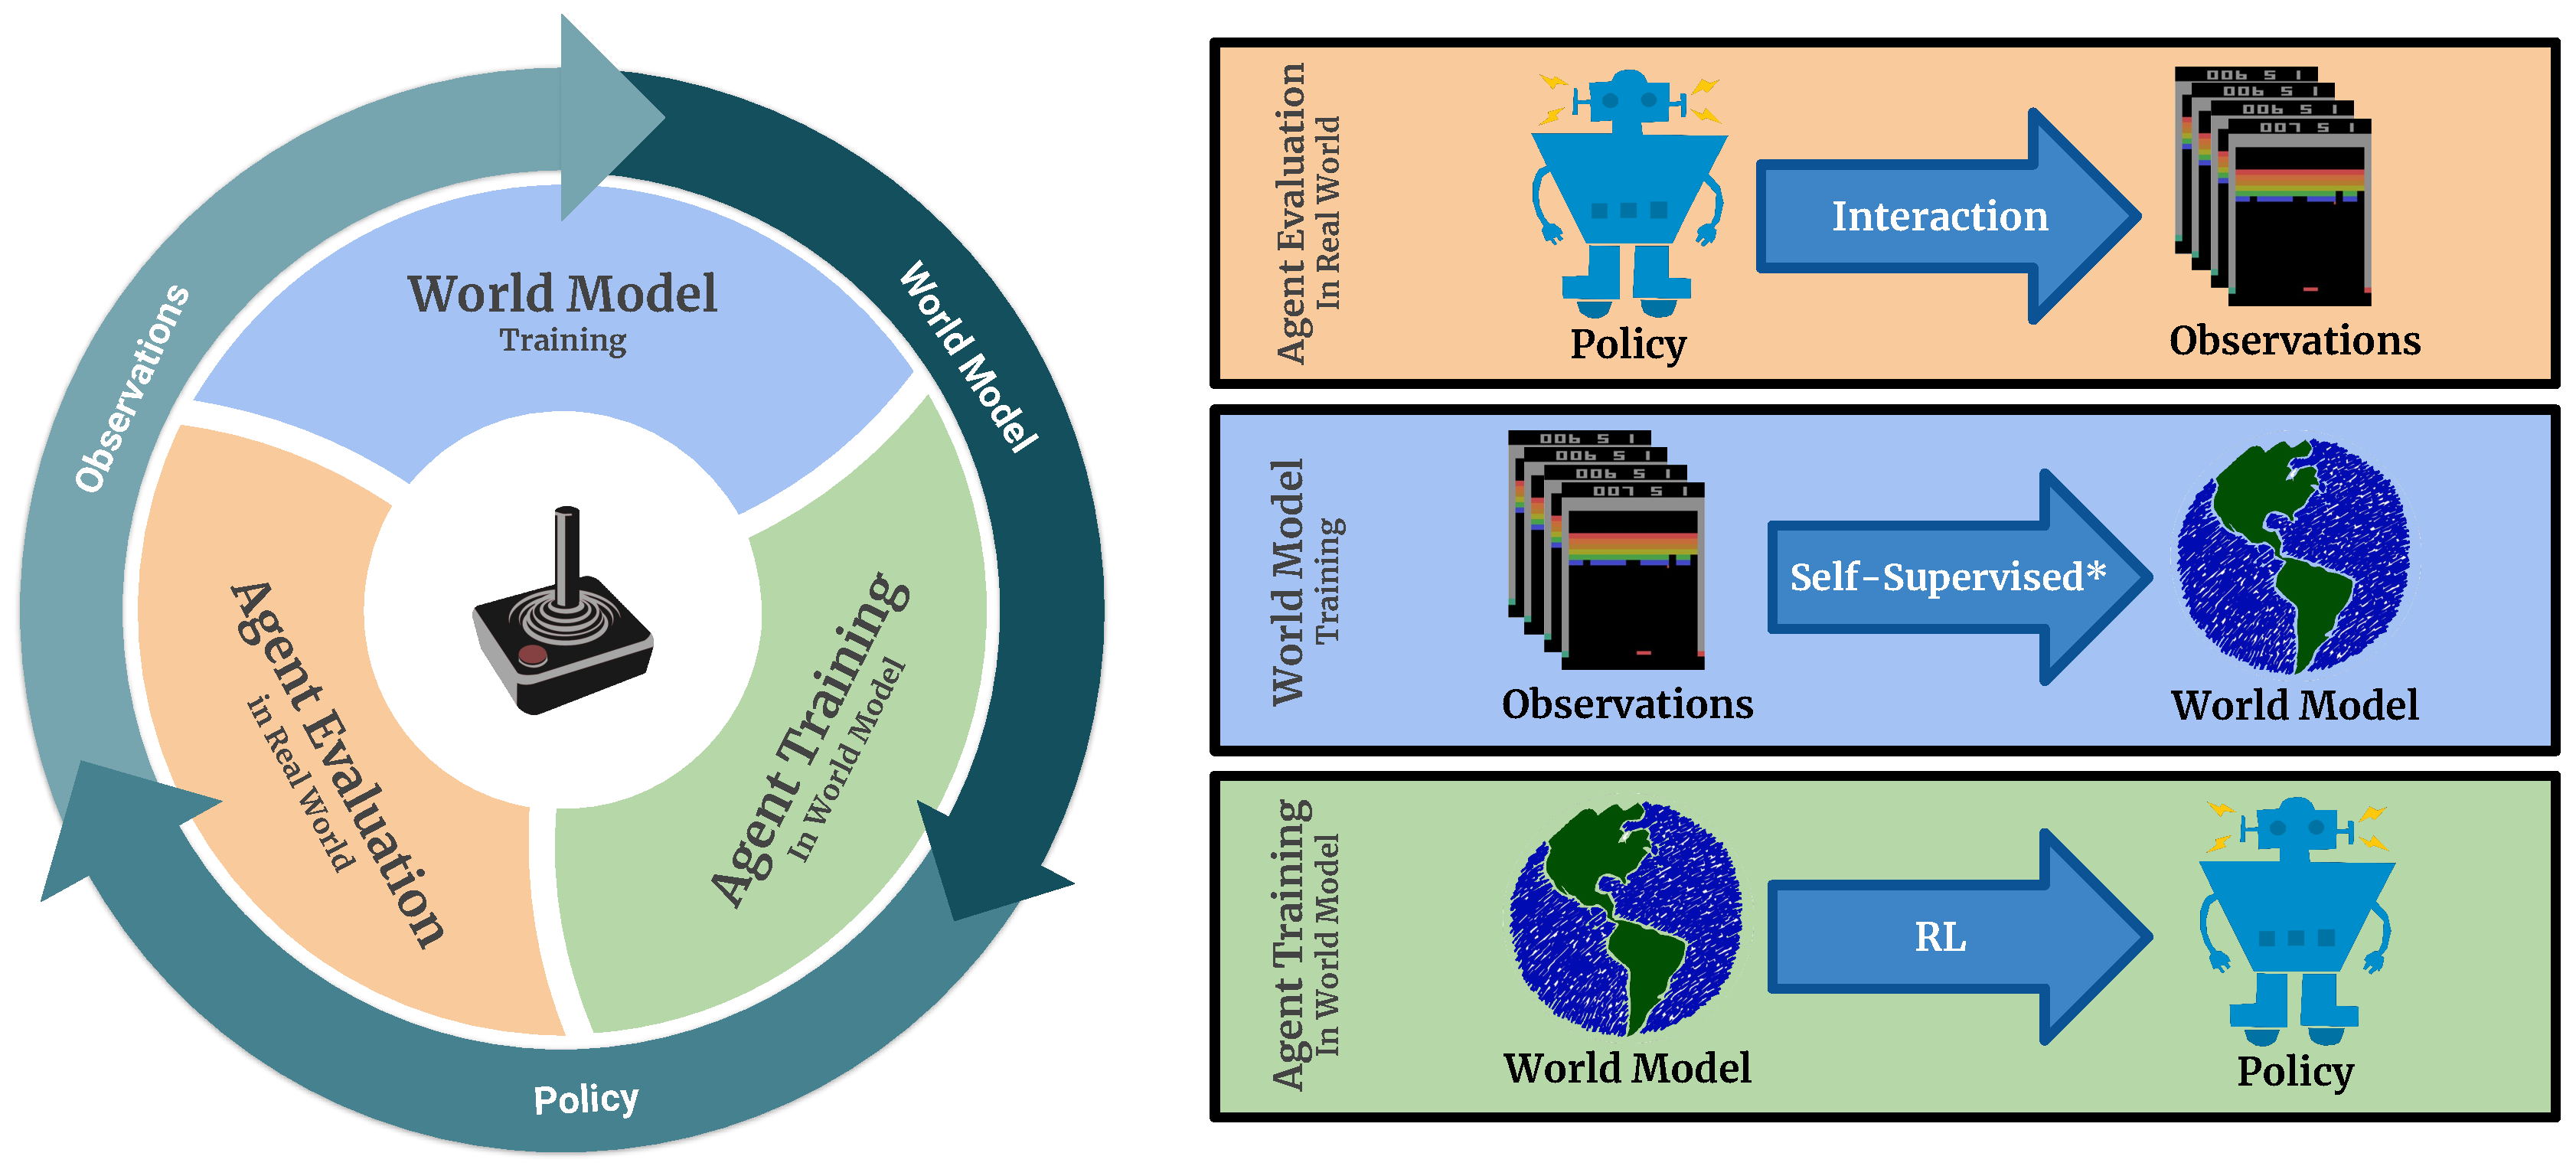
\includegraphics[width=1.0\textwidth]{figures/Cycle_full.pdf}
\caption{Main loop of SimPLe. 1) the agent starts interacting with the real environment following the latest policy (initialized to random). 2) the collected observations will be used to train (update) the current world model. 3) the agent updates the policy by acting inside the world model. The new policy will be evaluated to measure the performance of the agent as well as collecting more data (back to 1).  Note that world model training is self-supervised for the observed states and supervised for the reward.}
\label{fig:main_cycle}
\end{figure*}
